% Chapter 4
\label{Capítulo4}
\chapter{Implementação}
\begin{center}
	\textit{``Do or do not. There is no try.''}

	Master Yoda
\end{center}
Neste capítulo aborda-se com mais pormenor os aspectos mais técnicos do \acrshort{lare}, tendo como base a arquitectura apresentada na Figura \ref{fig:arquitecturalore}.

O desenvolvimento começou pela implementação e desenvolvimento do servidor \textit{Flask} e página \textit{web}. O primeiro circuito a ser testado e integrado foi a Lei de Ohm. O projecto foi evoluindo com a adição dos restantes circuitos que compõem o \acrshort{lare}.

O \acrshort{ide} utilizado no desenvolvimento do \textit{software} foi o \textit{Visual Studio Code}\footnote{\url{https://code.visualstudio.com/}} e o projecto está alojado no \textit{GitHub}. O sistema operativo instalado no RaspberryPI 5 foi uma versão ligeiramente modificada do \textit{Arch Linux ARM}.

Os circuitos que compõem o \acrshort{lare} foram testados e validados individualmente em placas brancas, antes de se proceder à construção da matriz de placas, como referido na Secção \ref{sec:matriz}.

\section{Software}
\subsection{Servidor Flask}
\label{sec:flask}
\textbf{Não sei se ainad vai ficar desta forma}

Hoje em dia vive-se (n)uma Era em que toda a informação está disponível na ``ponta dos dedos'' e à distância de um \textit{click}. A pesquisa, desenvolvimento e teste dos assuntos mais técnicos revelou-se longa e muitas vezes extenuante. Os recursos são (quase) incomensuráveis e o grande desafio é tentar perceber a dicotomia certo/errado. Recorreu-se à Inteligência Artificial, documentação técnica \textit{online}, fóruns de discussão, ajuda pessoal, tutoriais \textit{online} e vídeos no YouTube.

A base para a implementação do \textit{Flask} e \underline{\textbf{toda a informação descrita neste}} \underline{\textbf{capítulo}} teve como base a documentação técnica disponível no \textit{site} do \href{https://flask.palletsprojects.com/en/3.0.x/}{\textit{Flask}} e complementada com alguns tutoriais do \textit{Youtube}, como por exemplo: \href{https://www.youtube.com/watch?v=dam0GPOAvVI}{\textit{link}} ou \href{https://www.youtube.com/watch?v=bB6Yyh7nUl4}{\textit{link}} .

\subsubsection{Estrutura base}
O fluxograma apresentado na Figura \ref{fig:funcflask} apresenta o funcionamento geral do servidor \textit{Flask}.

\begin{figure}[hbtp]
	\centering
	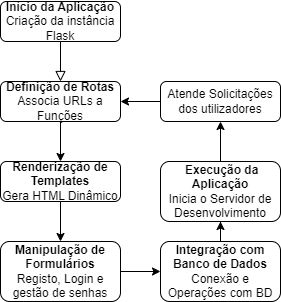
\includegraphics[width=0.7\textwidth]{figures/fluxograma_flask.drawio.png}
	\caption{Funcionamento geral \textit{Flask}}
	\label{fig:funcflask}
\end{figure}

A estrutura de directórios do \textit{Flask} tem uma base pré-definida que não é necessariamente rígida e pode ser adaptada consoante os requisitos do projecto \cite{Flask}. No caso do \acrshort{lare} a estrutura ficou organizada da forma como se mostra na Figura \ref{fig:estruturapastas}

\begin{figure}[hbtp]
	\centering
	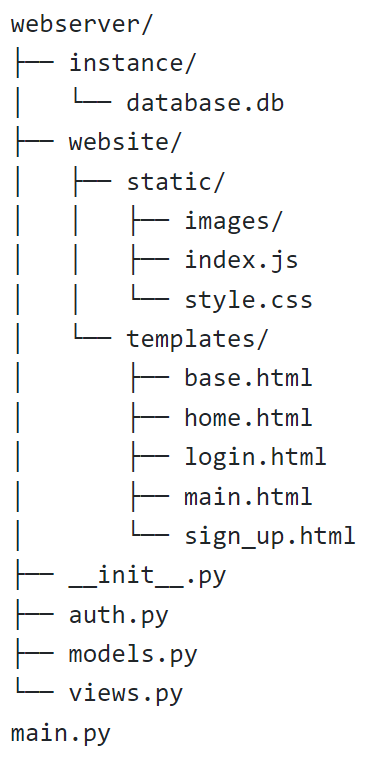
\includegraphics[width=0.3\textwidth]{figures/tree_flask.png}
	\caption{Estrutura de directórios - \textit{Flask} \textbf{ main.html está a mais}}
	\label{fig:estruturapastas}
\end{figure}

A raiz do projecto é o directório ``\textit{webserver}'' e nele estão contidos o ficheiro principal, assim como outros directórios e ficheiros de configuração essenciais:
\begin{itemize}
	\item \textit{main.py}: O ficheiro principal do aplicativo que inicializa e configura o \textit{Flask};
	\item \textit{requirements.txt}: Uma lista de dependências do projeto que podem ser instaladas usando \gls{pip};
	\item \textit{static/}: Este diretório contém os ficheiros estáticos como \acrshort{css}, \textit{JavaScript} e as imagens usadas em toda a aplicação;
	\item \textit{templates/}: Contém os modelos \acrshort{html} usado para renderizar as visualizações;
	\item \textit{instance/}: Diretório para armazenar ficheiros de configuração ou ficheiros que mudam em tempo de execução, específicos da cada instância, por exemplo, ficheiros da base de dados.
\end{itemize}

Dentro da raiz, criou-se o directório \textit{website} onde se incluiu os ficheiros respeitantes ao funcionamento do \textit{site}. Nele constam os já descritos \textit{templates}, \textit{static} e ainda os seguintes ficheiros:

\begin{itemize}
	\item \textit{\_\_init\_\_.py}: Inicializa o \textit{Flask} e define as configurações. Este ficheiro dentro da directoria \textit{website} faz com que esta seja tratada como um pacote \textit{Python}. Isto quer dizer que a directoria pode ser importada e tudo o que estiver dentro é executado automaticamente;
	\item \textit{views.py}: Contém as funções de visualização para o tratamento de pedidos \acrfull{http};
	\item \textit{models.py}: Define os modelos de dados para a aplicação;
	\item \textit{auth.py}: Este ficheiro é responsável por lidar com a autenticação e autorização de utilizadores, pode incluir funções e rotas que permitem aos utilizadores registarem-se, fazer \textit{login} e fazer \textit{logout}.
\end{itemize}

\subsubsection{Rotas}
As aplicações \textit{Web} modernas utilizam \acrshort{url}s amigáveis para ajudar os utilizadores a memorizar e utilizar o nome para voltar a visitar diretamente uma página.

No \textit{Flask} utiliza-se o decorador \textit{\textbf{route()}} para associar uma função a um \acrshort{url}, tal como pode ser visto na Listagem \ref{lst:decoradorroute}.

\begin{minipage}{0.9\linewidth}
	\begin{lstlisting}[language=Python, caption=Decorador \textit{route()} - \textit{views.py}, label=lst:decoradorroute]
@views.route("/ohm", methods=['GET', 'POST'])
@login_required
def pagina_seguinte():
    return render_template("ohm.html", user=current_user)
\end{lstlisting}
\end{minipage}

O decorador \textit{\textbf{route}} define uma rota para a \acrshort{url} \textit{ohm}. Esta rota aceita pedidos \acrshort{http} de métodos \textit{GET} e \textit{POST}.

O decorador \textit{\textbf{login}} garante que o utilizador tem de estar autenticado para aceder a esta rota. Se o utilizador não estiver autenticado, será redirecionado para a página de \textit{login}.

A função pagina\_seguinte() é executada assim que a respectiva rota for acedida.

A última linha renderiza o \textit{template} \textit{\textbf{home.html}} e passa o objecto \textit{current\_user} para o \textit{template}.

Para construir um \acrshort{url} para uma função específica, usa-se a função \textit{\textbf{url\_for()}}. Esta função aceita o nome da função como seu primeiro argumento e qualquer número de argumentos de palavras-chave, cada um correspondendo a uma parte variável da regra de \acrshort{url}, tal como pode ser visto na Listagem \ref{lst:urlfor}

\begin{minipage}{0.9\linewidth}
	\begin{lstlisting}[language=Python, caption=Contrução de \textit{url}s - \textit{auth.py}, label=lst:urlfor]
(...)
if user:
    if check_password_hash(user.password, password):
        flash('Logged in successfully!', category='success')
        login_user(user, remember=True)
        return redirect(url_for('views.home'))
(...)
\end{lstlisting}
\end{minipage}

Isto quer dizer que o \textit{Flask} gera a \acrshort{url} correspondente à função \textit{\textbf{home()}} definida no ficheiro \textit{\textbf{views.py}} dentro da \textit{Blueprint} \textit{views}. Quando usada dentro de \textit{\textbf{redirect}}, redireciona o utilizador para essa \acrshort{url}.

\subsubsection{Blueprints}
O \textit{Flask} usa um conceito de \textit{blueprints} para criar componentes de aplicações e suportar padrões comuns dentro de uma aplicação ou entre aplicações. As \textit{blueprints} podem simplificar muito o funcionamento de grandes aplicações e fornecer um meio central para que as extensões do \textit{Flask} registem operações em aplicações. As \textit{blueprints} permitem organizar a aplicação em partes menores e de mais fácil gestão. O conceito básico das \textit{blueprints} é que registam as operações a executar quando são integrados numa aplicação. O \textit{Flask} associa funções de vista (\textit{views}) a \textit{blueprints} quando processa pedidos e gera \acrshort{url} entre diferentes pontos de acesso.

Nas Listagens \ref{lst:blueprintviews} e \ref{lst:blueprintauth} podem ver-se as duas \textit{blueprints} definidas no caso da implementação do \acrshort{lare}.
\begin{center}
	\begin{minipage}{0.7\linewidth}
		\begin{lstlisting}[language=Python, caption=\textit{Blueprint views} - \textit{views.py}, label=lst:blueprintviews]
views = Blueprint('views', __name__)
\end{lstlisting}
	\end{minipage}
\end{center}

\begin{center}
	\begin{minipage}{0.7\linewidth}
		\begin{lstlisting}[language=Python, caption=\textit{Blueprint auth} - \textit{auth.py}, label=lst:blueprintauth]
auth = Blueprint('auth', __name__)
\end{lstlisting}
	\end{minipage}
\end{center}

Ambas as \textit{blueprints} são registadas no ficheiro \textit{\_\_init\_\_.py}, como se pode verificar na Listagem \ref{lst:initreg}

\begin{center}
	\begin{minipage}{0.7\linewidth}
		\begin{lstlisting}[language=Python, caption=Registo das \textit{blueprints} - \textit{\_\_init\_\_.py}, label=lst:initreg]
app.register_blueprint(views, url_prefix='/')
app.register_blueprint(auth, url_prefix='/')
\end{lstlisting}
	\end{minipage}
\end{center}

Isto quer dizer que ao registar a \textit{blueprint} com o prefixo ``/'', os \acrshort{url}s serão acessíveis através da raiz da aplicação.

\subsubsection{Pedidos}
A capacidade de uma aplicação \textit{web} em responder a solicitações de dados do cliente é um requisito essencial. No \textit{Flask} esta informação é fornecida pelo objeto global \textit{\textbf{request}}. Este objeto contém todos os detalhes da solicitação, como os métodos \acrshort{http} usados (\textit{GET}, \textit{POST}, etc.), os \textit{headers} os \textit{cookies} ou o corpo da requisição.

O método de requisição pode ser determinado através do atributo \textit{\textbf{method}}. Para aceder aos dados de um formulário (transmitidos numa requisição \textit{POST} ou \textit{PUT}), utiliza-se o atributo \textit{\textbf{form}}, tal como pode ser visto na Listagem \ref{lst:atributorequest}.

\begin{minipage}{0.9\linewidth}
	\begin{lstlisting}[language=Python, caption=Exemplo atributo \textit{\textbf{request} - \textit{auth.py}}, label=lst:atributorequest]
@auth.route('/login', methods=['GET', 'POST'])
def login():
    if request.method == 'POST':
        email = request.form.get('email')
        password = request.form.get('password')

        user = User.query.filter_by(email=email).first()
        if user:
            if check_password_hash(user.password, password):
                flash('Logged in successfully!', category='success')
                login_user(user, remember=True)
                return redirect(url_for('views.home'))
            else:
                flash('Incorrect password, try again.', category='error')
        else:
            flash('Email does not exist.', category='error')

    return render_template("login.html", user=current_user)
\end{lstlisting}
\end{minipage}

Quando se adiciona um ponto de interrogação (?) seguido de pares chave-valor (key=value) no final de um \acrshort{url}, está a enviar-se dados adicionais ao servidor, esses dados são chamados de \textbf{parâmetros do \acrshort{url}}, como se pode ver na Listagem \ref{lst:paramurl}.

\begin{minipage}{0.9\linewidth}
	\begin{lstlisting}[language=Python, caption=Exemplo atributo \textit{\textbf{args} - \textit{views.py}}, label=lst:argrequest]
@views.route('/config_VirtualBench', methods=['GET', 'POST'])
@login_required
def config_VirtualBench():
    try:
        Vcc = request.args.get('Vcc', 0, int)
        Resistance = request.args.get('R', 0, int)
        (...)
    except Exception as e:
        print(e)
        return jsonify({'measurement_result': 'ERROR'})
    finally:
        return jsonify({'measurement_result': measurement_result})
\end{lstlisting}
\end{minipage}

\begin{minipage}{0.9\linewidth}
	\begin{lstlisting}[language=Html, caption=Exemplo argumentos passados ao servidor - ohm.html, label=lst:paramurl]
const url = `/config_VirtualBench?parameter=${parameter}&Vcc=${Vcc}&R=${Resistance}`;
\end{lstlisting}
\end{minipage}

No entanto, a criação e renderização das páginas \acrshort{html} é feita automaticamente através dos modelos \textit{Jinja2}\footnote{A documentação pode ser consultada em \href{https://jinja.palletsprojects.com/en/3.1.x/templates/}{\textit{Jinja}}}. Os modelos podem ser usados para gerar qualquer tipo de ficheiro de texto, sendo que para aplicações \textit{web} serão, principalmente, páginas \acrshort{html}.

Na Listagem \ref{lst:htmljinja2} pode ver-se um exemplo da combinação entre código \acrshort{html} e sintaxe \textit{Jinja2}.

\begin{minipage}{0.9\linewidth}
	\begin{lstlisting}[language=Html, caption=Exemplo sintaxe \textit{Jinja2} - base.html, label=lst:htmljinja2]
<title>Home</title>
  </head>
  <body>
    <nav class="navbar navbar-expand-lg navbar-dark bg-dark">
      <button
        class="navbar-toggler"
        type="button"
        data-toggle="collapse"
        data-target="#navbar"
      >
        <span class="navbar-toggler-icon"></span>
      </button>
      <div class="collapse navbar-collapse" id="navbar">
        <div class="navbar-nav">
          
          <a class="nav-item nav-link" id="home" href="/">Home</a>
          <a class="nav-item nav-link" id="logout" href="/logout">Logout</a>
          
          <a class="nav-item nav-link" id="login" href="/login">Login</a>
          <a class="nav-item nav-link" id="signUp" href="/sign-up">Sign Up</a>
          
        </div>
      </div>\end{lstlisting}
\end{minipage}

No código \acrshort{html}, encontram-se secções entre chavetas {} com palavras-chave especiais como por exemplo {\% block \%} e {\% endblock \%}. Estes são blocos de modelo \textit{Jinja2} que definem áreas de conteúdo dinâmico que podem ser preenchidas com lógica ou dados em \textit{Python}.

Para renderizar um modelo, o método utilizado foi \textit{\textbf{render\_template()}}, como pode ser visto na Listagem \ref{lst:atributorequest}, linha 18. O \textit{Flask} procurará por modelos na pasta \textit{templates}, como pode ser visto na Figura \ref{fig:estruturapastas}.

Na página oficial do \textit{Flask} é recomendado que se aceda aos parâmetros do \acrshort{url} com \textit{\textbf{get}} ou capturando o \textit{\textbf{KeyError}}, uma vez que os utilizadores podem alterar o \acrshort{url} e, nesse caso, apresentar uma página \textit{400 bad request} não é de fácil interpretação.

\subsubsection{Base de dados}
A aplicação desenvolvida usa uma base de dados e autenticação de utilizador, a ligação com a base de dados é aberta no início do pedido e é obtida a informação do utilizador. No final do pedido, a ligação com a base de dados é fechada.

No contexto da documentação do \textit{Flask} e implementação de uma base de dados, são apresentados duas alternativas: \textit{SQLite 3} e \textit{ SQLAlchemy}. Tal como referenciado/aconselhado na documentação, usou-se a extensão \textit{Flask-SQLAlchemy}, como apresentado na Listagem \ref{lst:basedados}

\textbf{Nota para minha referência: Falar de instalar o pacote SQLAlchemy?}

\begin{minipage}{0.9\linewidth}
	\begin{lstlisting}[language=Python, caption=Exemplo uso \textit{ SQLAlchemy} - \textit{\_\_init.py\_\_}, label=lst:basedados]

from flask_sqlalchemy import SQLAlchemy

db = SQLAlchemy()
DB_NAME = "database.db"

def create_app():
    app = Flask(__name__)
    app.config['SECRET_KEY'] = 'hjshjhdjah kjshkjdhjs'
    app.config['SQLALCHEMY_DATABASE_URI'] = f'sqlite:///{DB_NAME}'
    db.init_app(app)
(...)
\end{lstlisting}
\end{minipage}

\subsubsection{Autenticação}
A segurança da aplicação é feita com recurso à página de \textit{login} e \textit{logout}, para isso foi instalada a extensão \textit{flask-login}, tal como é apresentado na Listagem \ref{lst:exemplologin}

\begin{minipage}{0.9\linewidth}
	\begin{lstlisting}[language=Python, caption=Exemplo autenticação \textit{login}, label=lst:exemplologin]
@auth.route('/login', methods=['GET', 'POST'])
def login():
    if request.method == 'POST':
        email = request.form.get('email')
        password = request.form.get('password')

        user = User.query.filter_by(email=email).first()
        if user:
            if check_password_hash(user.password, password):
                flash('Logged in successfully!', category='success')
                login_user(user, remember=True)
                return redirect(url_for('views.home'))
            else:
                flash('Incorrect password, try again.', category='error')
        else:
            flash('Email does not exist.', category='error')
    return render_template("login.html", user=current_user) 
\end{lstlisting}
\end{minipage}

\section{pyVirtualBench}
\label{sec:pyvirtualbench}
Antes de se avançar para uma explicação mais pormenorizada das experiências, importa enquadrar o \textit{pyVirtualBench} no contexto do \textit{software}. Já foi referido na Secção \ref{sec:solucaoproposta} que o \textit{pyVirtualBench} é um \textit{wrapper} que permite controlar o \acrshort{virtualbench} a partir de uma aplicação \textit{Python}. Viu-se também que este \textit{wrapper} não é compatível com \textit{Linux} e não é suportado oficialmente pela \acrshort{ni}. Por isso, toda a programação, controlo e configuração do \acrshort{virtualbench} foi realizada com base neste \textit{wrapper} que pode ser transferido ou consultado no \href{https://github.com/armstrap/armstrap-pyvirtualbench/tree/master}{GitHub}.

Além de instalar a biblioteca, os autores disponibilizam uma série de exemplos, sendo que, aqueles que mais se enquadram nos objectivos deste projecto são:
\begin{itemize}
	\item \textit{dmm\_example.py}: exemplo que demonstra como efetuar medições utilizando o multímetro digital;
	\item \textit{fgen\_example.py}: exemplo que demonstra como configurar e gerar uma onda através do gerador de sinal;
	\item \textit{mso\_simple\_example.py}: exemplo que demonstra como configurar e adquirir dados do osciloscópio, utilizando a funcionalidade de configuração automática incorporada;
	\item \textit{ps\_example.py}: exemplo que demonstra como efetuar medições utilizando a fonte de alimentação.
\end{itemize}

\subsection{VirtualBench VB-8012}
\label{sec:VB8012}
Na implementação do \textit{pyVirtualBench} é preciso ter em atenção alguns pormenores que podem levantar potenciais problemas de interpretação e implementação.

Como já se viu na Secção \ref{sec:hardware} o \acrshort{virtualbench} é constituído por 5 instrumentos, 4 dos quais utilizados no \acrshort{lare}: Fonte de tensão, gerador de sinal, osciloscópio e multímetro digital.
Vários instrumentos podem ser chamados ao mesmo tempo e a cada instrumento, assim como ao \acrshort{virtualbench} é atribuído um \textbf{OBJECTO?endereço?referência? - verificar}
\begin{center}
	\begin{minipage}{0.75\linewidth}
		\begin{lstlisting}[language=Python, caption=Chamada do \acrshort{virtualbench} e instrumentos, label=lst:chamadainstrumentos]
virtualbench = PyVirtualBench('VB8012-30A210F')
ps = virtualbench.acquire_power_supply()
dmm = virtualbench.acquire_digital_multimeter()
\end{lstlisting}
	\end{minipage}
\end{center}

O resultado da Listagem \ref{lst:chamadainstrumentos} é:
\begin{itemize}
	\item (...)PyVirtualBench object at 0x000001E7DEECAD20.
	\item (...)PyVirtualBench.PowerSupply object at 0x000001E7DEECB2F0;
	\item (...)PyVirtualBench.DigitalMultimeter object at 0x000001E7DEECBC50;
\end{itemize}

No entanto, no fim da execução do ficheiro, o \acrshort{virtualbench} e os restantes instrumentos têm de ser libertados:
\begin{center}
	\begin{minipage}{0.75\linewidth}
		\begin{lstlisting}[language=Python, caption=Libertar instrumentos e \acrshort{virtualbench}, label=lst:libertarinstrumentos]
ps.release()
dmm.release()
virtualbench.release()
\end{lstlisting}
	\end{minipage}
\end{center}

Sempre que o ficheiro é chamado é criado um objecto diferente para cada instrumento. Inclusive, havendo várias funções no mesmo ficheiro, os objectos criados têm de ser passados entre funções ou então, terminar e chamar o(s) instrumento(s) entre chamadas de funções. Outra hipótese seria o uso de variáveis globais. Estes factos/procedimentos/whetever levantariam problemas de objectividade e organização do código.

Na secção seguinte explica-se a solução encontrada.

\section{Hardware}
\subsection{Circuitos/Experiências}
\label{sec:experiencias}
Como já foi referido na Secção \ref{sec:solucaoproposta}, o \acrshort{lare} é composto por 5 circuitos. A implementação começou com o desenho esquemático e, tal como referido na Secção \ref{sec:reles}, tentou-se, sempre que possível, utilizar os relés \acrshort{spst} no comando das fontes e aparelhos de medida e os relés \acrshort{dpst} no controlo dos componentes, tal como se pode ver na Figura \ref{fig:relespstdpst}. O relé \textit{K4} - \acrshort{spst} - comanda a fonte de alimentação de \SI{5}{\volt} e os relés \textit{K1} a \textit{K3} - \acrshort{dpst} - comandam os componentes.

\begin{figure}[hbtp]
	\centering
	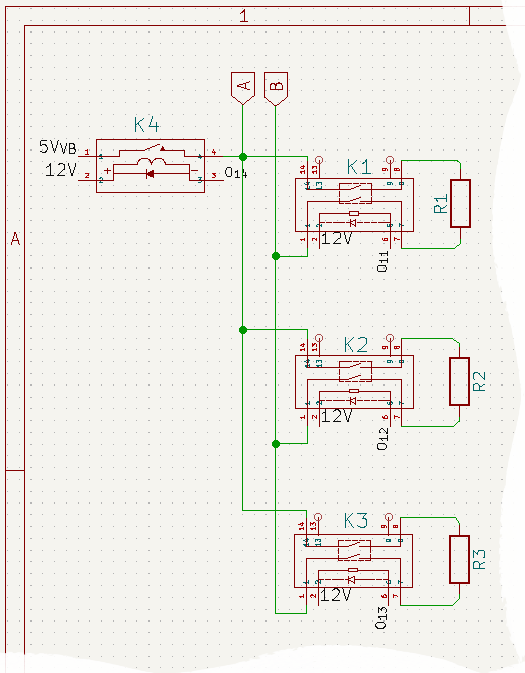
\includegraphics[width=0.6\textwidth]{figures/exemplo_reles_spst.png}
	\caption{Exemplo de utilização de relés \acrshort{spst} e \acrshort{dpst}}
	\label{fig:relespstdpst}
\end{figure}

Como já foi referido na Secção \ref{sec:registodeslocamento}, o \textit{SN74HC595} é um registo de deslocamento de 8 \textit{bits}, do tipo \acrshort{sipo}. Uma trama de (até 8) \textit{bits} é enviado pelo \gls{RaspberryPI} para o registo através do pino \acrshort{ser}. Na Figura \ref{fig:esquematico74hc595} pode ver-se o diagrama explicativo do processo de envio:

\begin{enumerate}
	\item Pinos \acrshort{oe} e \acrshort{srclr} activados;
	\item Um \textit{bit} ``0'' ou ``1'' é enviado para o pino \acrshort{ser};
	\item \textit{N} impulsos ascendentes no pino \acrshort{srclk} fazem com que o \textit{N bits} sejam enviado para o registo de deslocamento (\textit{N bits} <= 8);
	\item Um impulso ascendente no pino \acrshort{rclk} faz com que os \textit{N bits} sejam enviados para o registo de memória e, por conseguinte, para os relés (através do \textit{ULN2003A}).
\end{enumerate}

%Por cada impulso ascendente no pino \textit{SRCLK} - \textit{Shift Register Clock} - Os \textit{bits} são enviados um-a-um para o registo de deslocamento. No final, um impulso ascendente no \textit{RCLK} - \textit{Register Clock} - faz com que os \textit{bits} sejam enviados para o registo de memória e, por conseguinte, para os relés.

\begin{figure}[hbtp]
	\centering
	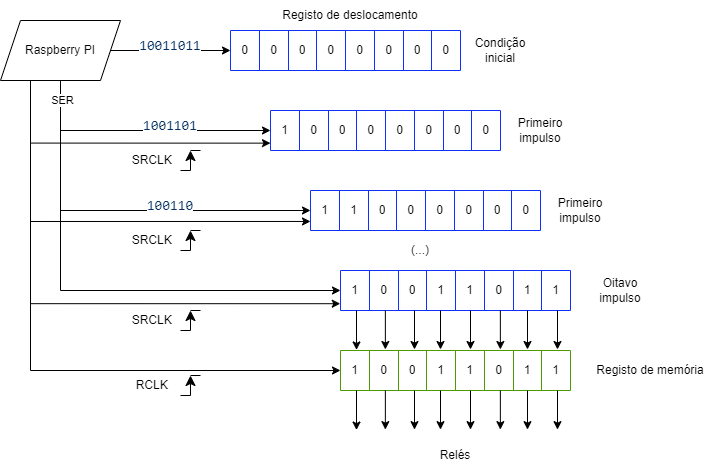
\includegraphics[width=1\textwidth]{figures/registo deslocamente.drawio.png}
	\caption{Envio de \textit{bits} para o registo de deslocamento}
	\label{fig:esquematico74hc595}
\end{figure}

Foi referido na Secção \ref{sec:driver}, que o \gls{RaspberryPI} não tem capacidade para comandar os relés. Para isso, é necessário usar o \textit{ULN2003A} que é um \textit{driver} de relés. Na Figura \ref{fig:diagramablocos2003} está representado o diagrama simplificado para uma entrada/saída do \textit{ULN2003A} \cite{ULN2003}.

\begin{figure}[hbtp]
	\centering
	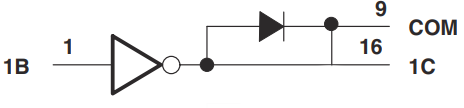
\includegraphics[width=0.6\textwidth]{figures/uln2003_diagramablocos.png}
	\caption{Diagrama de blocos simplificado do \textit{ULN2003A}}
	\label{fig:diagramablocos2003}
\end{figure}

O terminal 9 - \textit{COM} - é ligado à tensão de comando dos relés e é destinado aos díodos de ``roda livre'', conforme mencionado na Secção \ref{sec:reles}. No caso dos modelos de relés utilizados neste projecto, a tensão é de \SI{12}{\volt}.
O \textit{ULN2003A} faz parte da família dos \textit{drivers} inversores. Se o valor lógico na entrada ``1B'' = ``0'' (ou \SI{0}{\volt}), então, a saída ``1C'' = ``1'' (ou \SI{12}{\volt}).

As Figuras \ref{fig:comandorelesfull} e \ref{fig:exemplovoltimetro} servem como exemplo para ilustrar o funcionamento dos relés, em conjunto com o \textit{ULN2003A} e o \textit{SN74HC595}. Neste exemplo usou-se um relé \acrshort{spst}. No entanto, o funcionamento é idêntico para os relés \acrshort{dpst}, mudando somente os pinos.

\begin{figure}[hbtp]
	\centering
	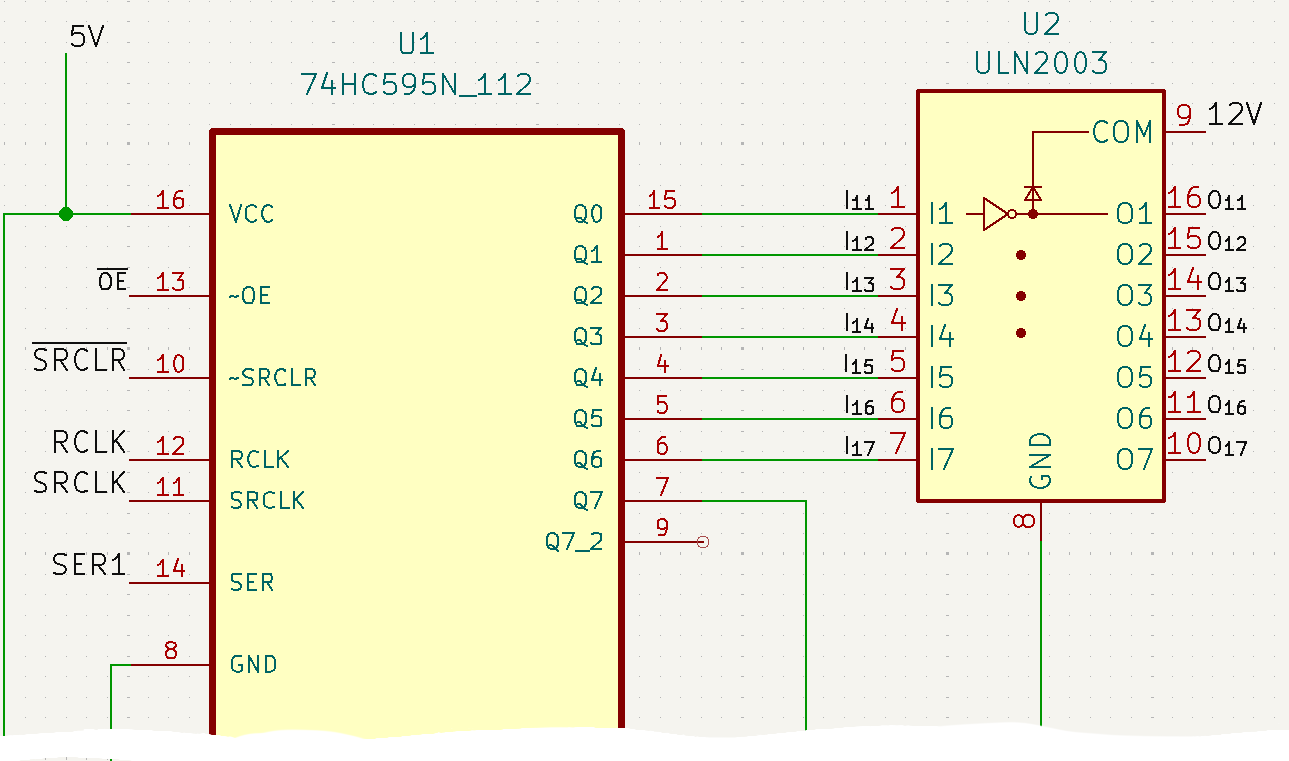
\includegraphics[width=0.7\textwidth]{figures/comandoreles_FULL.png}
	\caption{Exemplo de uso do \textit{SN74HC595} e \textit{ULN2003A} - REVER}
	\label{fig:comandorelesfull}
\end{figure}

\begin{figure}[hbtp]
	\centering
	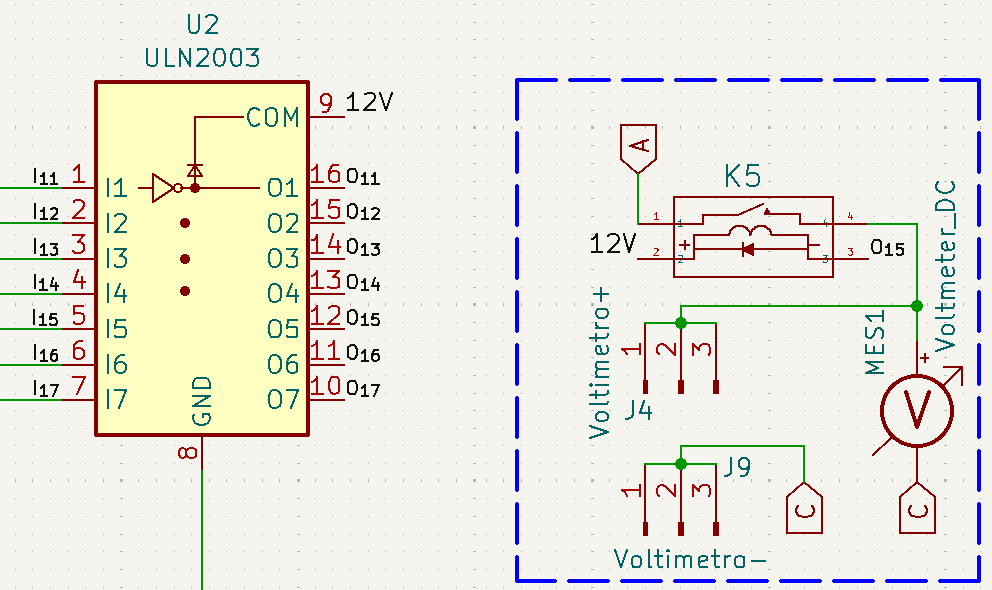
\includegraphics[width=0.7\textwidth]{figures/exemplo_voltimetro.png}
	\caption{Exemplo de comando dos relés, usando o \textit{ULN2003A}}
	\label{fig:exemplovoltimetro}
\end{figure}

As entradas $I_{1}$ a $I_{7}$ são comandadas pelo \gls{RaspberryPI}, através do registo de deslocamento - \textit{SN74HC595}, tal como apresentado na Figura \ref{fig:comandorelesfull} e as saídas $O_{1}$ a $O_{7}$ vão comandar os relés - terminais ``3'' e os terminais ``2'' dos relés são ligados aos \SI{12}{\volt}, como apresentado na Figura \ref{fig:exemplovoltimetro}.
%O funcionamento está descrito na Listagem \ref{Table:exemplouln2003}:

% \begin{table}[htb]
% 	\centering
% 	\caption{Tabela funcionamento \textit{ULN2003A} e relés}
% 	\label{Table:exemplouln2003}
% 	\begin{tabular}{ccc}
% 		\toprule
% 		\multicolumn{2}{c}{ULN2003A} & Relés                                \\
% 		\midrule
% 		Entrada                      & Saída                  & Estado      \\
% 		\midrule
% 		``0'' (\SI{0}{\volt})        & ``1'' (\SI{12}{\volt}) & Desactivado \\
% 		\midrule
% 		``1'' (\SI{12}{\volt})       & ``0'' (\SI{0}{\volt})  & Activado    \\
% 		\bottomrule
% 	\end{tabular}
% \end{table}

No caso particular do exemplo descrito em cima, se $I_{5} = I_{15}$ = \SI{0}{\volt}, então, a saída $O_{5}$ = \SI{12}{\volt} e não há diferença nos terminais ``2'' e ``3'' na bobina do relé  ``K5''. O relé está desactivado. Por outro lado, se $I_{5} = I_{15}$ = \SI{12}{\volt}, então, a saída $O_{5}$ = \SI{0}{\volt}, há diferença de potencial aos terminais da bobina e o relé está activado.

No caso em que a trama a ser transmitida for maior que 8 \textit{bits}, há a necessidade de usar mais do que um registo de deslocamento. Neste caso, o pino 9 - $Q_{H}'$ - do primeiro registo \textit{SN74HC595} é ligado ao pino \acrshort{ser} do segundo registo e assim sucessivamente.

\subsubsection{Lei de Ohm}
\label{sec:lei_ohm}
Nesta experiência pretende-se estudar a Lei de Ohm. Na Figura \ref{fig:esq_geral_ohm} está representado o esquema geral do circuito.

\begin{figure}[hbtp]
	\centering
	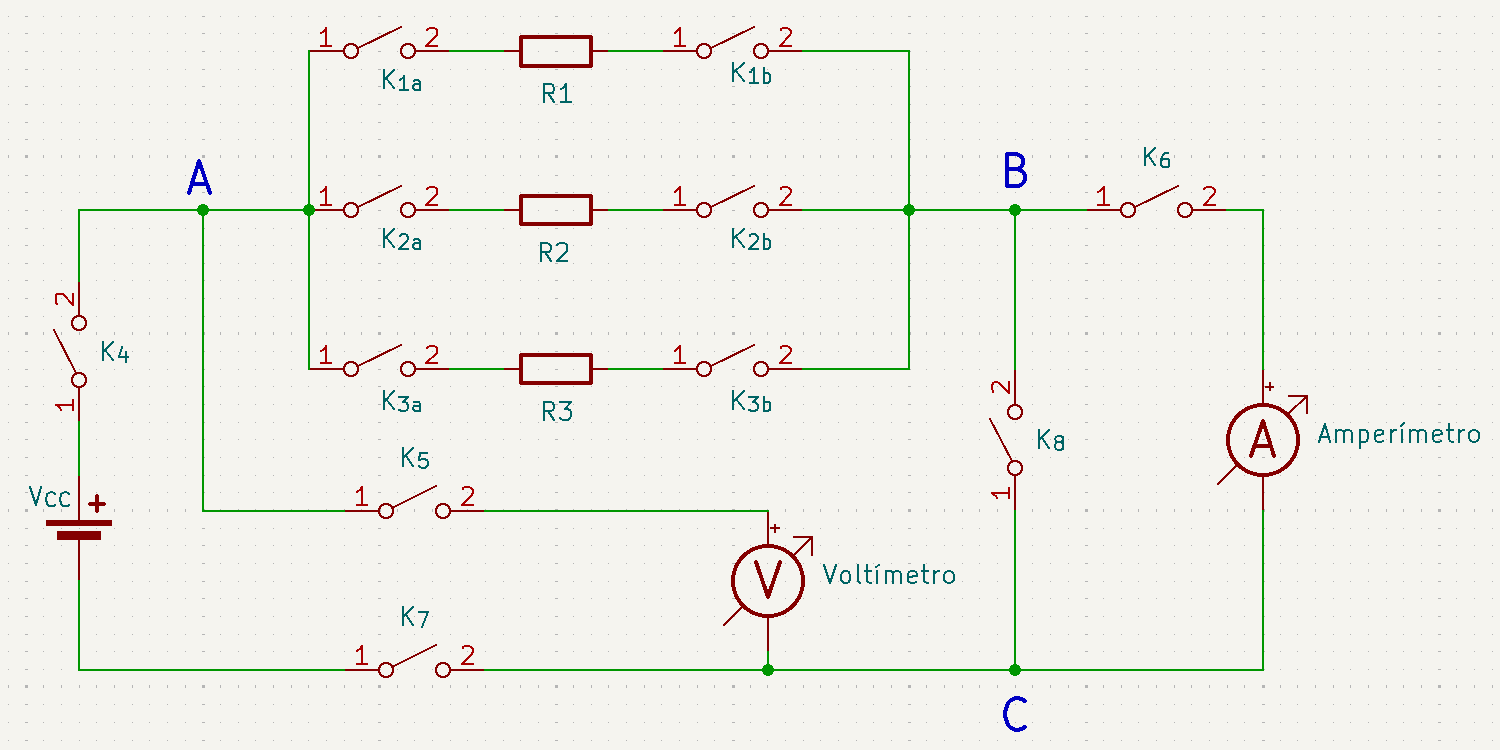
\includegraphics[width=1\textwidth]{figures/esquema_simplificado_OHM.png}
	\caption{Esquema geral da experiência Lei de Ohm}
	\label{fig:esq_geral_ohm}
\end{figure}

O funcionamento do circuito é relativamente simples. Qualquer que seja a resistência a medir, é fechado o respectivo relé - $K_{1}$ ou $K_{2}$ ou $K_{3}$; a fonte $V_{CC}$ é ligada ao circuito através do relé $K_{4}$ e $K_{7}$.

A medição da tensão e da corrente faz-se da seguinte forma:
\begin{itemize}
	\item Medição da tensão:
	      \begin{itemize}
		      \item Os relés $K_{5}$ e $K_{8}$ são fechados e $K_{6}$ é aberto. Desta forma, o voltímetro fica em paralelo com a resistência a medir - entre os pontos A e B.
	      \end{itemize}
	\item Medição da corrente:
	      \begin{itemize}
		      \item Os relés $K_{5}$ e $K_{8}$ são abertos e $K_{6}$ é fechado. Desta forma, o amperímetro fica em série com a resistência a medir - entre os pontos B e C.
	      \end{itemize}
\end{itemize}

Como se pode pode ver na Figura \ref{fig:frontDMM}, retirada da Figura \ref{fig:paineldianteiro}, o terminal preto (negativo) é comum a ambos os aparelhos de medida, que na Figura \ref{fig:esq_geral_ohm} está representado pelo ponto C. O terminal positivo do voltímetro liga ao ponto A - depois de activo o relé $K_{5}$ e o terminal positivo do amperímetro liga ao ponto B - depois de activo o relé $R_{6}$.

\begin{figure}[hbtp]
	\centering
	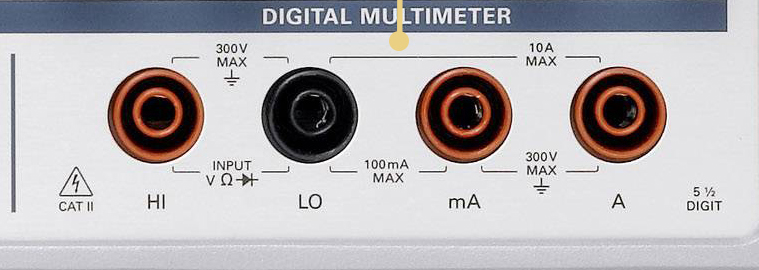
\includegraphics[width=1\textwidth]{figures/promenorDMM.png}
	\caption{Painel frontal Multímetro Digital}
	\label{fig:frontDMM}
\end{figure}

Por exemplo, se se pretender estudar a Lei de Ohm para a resistência $R_{1}$, os relés seriam activados da forma representada na Tabela \ref{Table:exemplomedicaoohm}:

\begin{table}[htb]
	\centering
	\caption{Exemplo funcionamento de medição da Lei de Ohm}
	\label{Table:exemplomedicaoohm}
	\begin{tabular}{lcccccccc}
		\toprule
		               & \multicolumn{8}{c}{Estado dos relés}                                                                       \\
		\midrule
		               & $K_{1}$                              & $K_{2}$ & $K_{3}$ & $K_{4}$ & $K_{5}$ & $K_{6}$ & $K_{7}$ & $K_{8}$ \\
		\midrule
		Medir Tensão   & 1                                    & 0       & 0       & 1       & 1       & 0       & 1       & 1       \\
		\midrule
		Medir Corrente & 1                                    & 0       & 0       & 1       & 0       & 1       & 1       & 0       \\
		\bottomrule
	\end{tabular}
\end{table}

De referir que, se se pretender expandir o \acrshort{lare} com mais circuitos, é possível utilizar o voltímetro e o amperímetro da forma como estão configurados. Tal como pode ser visto na Figura \ref{fig:esq_geral_ohm}, o voltímetro está disponível entre os pontos A e C e o amperímetro entre os pontos B e C.

\textbf{Colocar um exemplo de como ficariam os aparelhos de medida se o lare se expandisse com um circuito? OPINIÃO PROF}

Da forma como está implementado, o tutor ou professor, pode optar por apresentar o conceito de duas formas distintas:

\begin{itemize}
	\item O utilizador ou aluno parte do valor já conhecido da resistência e constrói o gráfico da Tensão \textit{vs} Corrente, efectuando cinco medições diferentes. No final confronta o valor conhecido com o declive da recta - que pode ser, ou não, apresentado com o gráfico, como pode ser visto na Figura \ref{fig:pagohm}.
	\item O utilizador ou aluno não sabe o valor da resistência e constrói o gráfico, obtendo o valor prático calculando o declive da recta, que mais uma vez, pode ou não, ser apresentado juntamente com o gráfico, tal como pode ser visto na Figura \ref{fig:pagohmabc}.
\end{itemize}

\begin{figure}[hbtp]
	\centering
	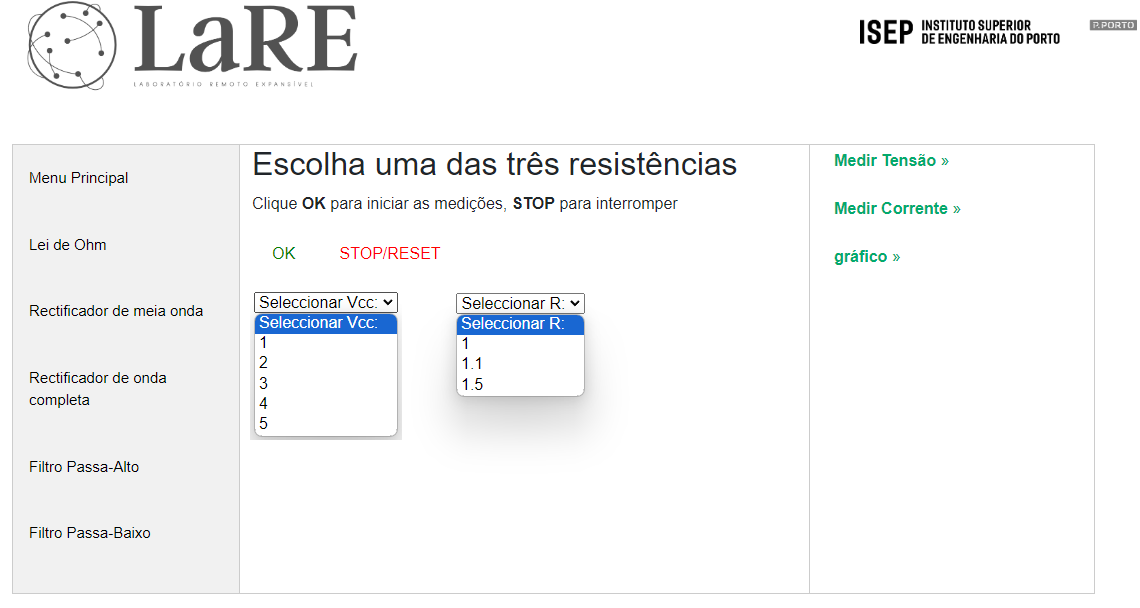
\includegraphics[width=1\textwidth]{figures/ohm_escolha.png}
	\caption{Experiência Lei de Ohm}
	\label{fig:pagohm}
\end{figure}

\begin{figure}[hbtp]
	\centering
	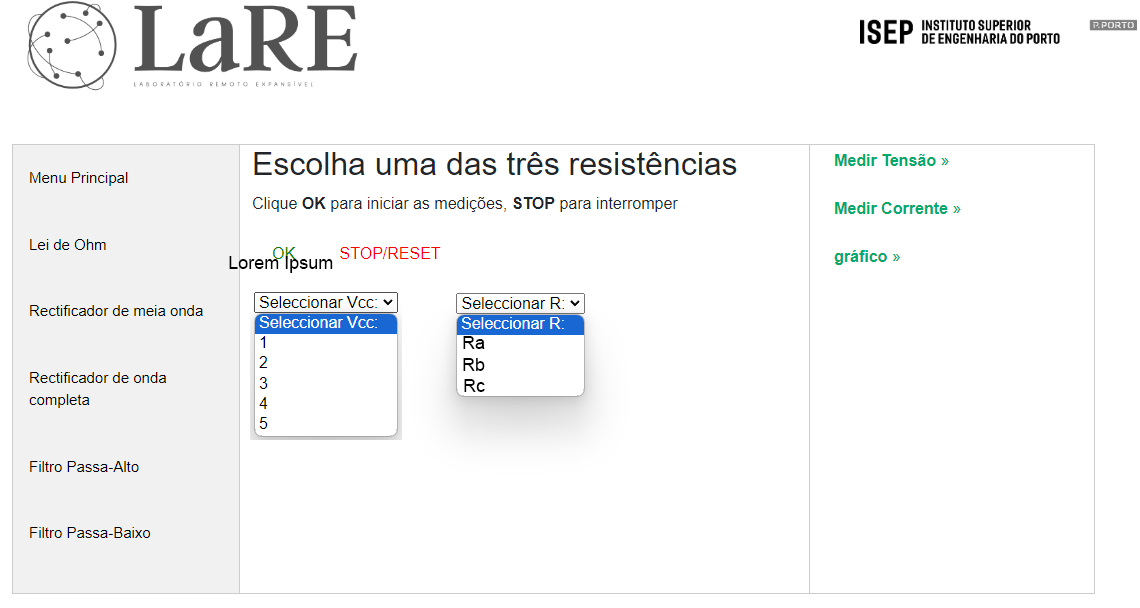
\includegraphics[width=1\textwidth]{figures/ohm_escolha_abc.png}
	\caption{Experiência Lei de Ohm - Resistências desconhecidas}
	\label{fig:pagohmabc}
\end{figure}

Devido à versatilidade e à liberdade que esta experiência proporciona, uma vez que, não só o utilizador ou aluno pode escolher a resistência e a ordem pela qual realiza as medições, mas também porque o professor ou tutor pode alterar os valores das tensões pré-definidas, esta experiência revelou-se, ao nível do \textit{software}, um desafio no que toca à sua implementação.

Como foi referido na Secção \ref{sec:pyvirtualbench}, alguns exemplos da biblioteca ``pyVirtualBench'' foram usados como base para o desenvolvimento da programação. Um desses exemplos é o que configura a fonte de tensão - \textit{ps\_example.py}.


\begin{minipage}{0.9\linewidth}
	\begin{lstlisting}[language=Python, caption=Exemplo \textit{ps\_example.py}, label=lst:exemplops]
		try:
			# Power Supply Configuration
			channel = "ps/+25V"
			voltage_level = 1.0
			current_limit = 0.5

			# You will probably need to replace "myVirtualBench" with the name of your device.
			# By default, the device name is the model number and serial number separated by a hyphen; e.g., "VB8012-309738A".
			# You can see the device's name in the VirtualBench Application under File->About
			virtualbench = PyVirtualBench('VB8012-30A210F')
			ps = virtualbench.acquire_power_supply()

			ps.configure_voltage_output(channel, voltage_level, current_limit)
			ps.enable_all_outputs(True)

			for i in range(10):
				voltage_measurement, current_measurement, ps_state = ps.read_output(channel)
				print("Measurement [%d]: %f V\t%f A\t(%s)" % (i, voltage_measurement, current_measurement, str(ps_state)))

			ps.release()
		except PyVirtualBenchException as e:
    		print("Error/Warning %d occurred\n%s" % (e.status, e))
		finally:
    		virtualbench.release()

	\end{lstlisting}
\end{minipage}

Como se pode ver na Listagem \ref{lst:exemplops}, o \textit{virtualbench} é chamado na linha 10 e a fonte de tensão na linha 11. O ciclo \textit{for}, na linha 16, executa uma série de 10 medições de tensão e corrente. A fonte é depois libertada, linha 20, e não havendo erro, o \textit{virtualbench} é libertado, linha 22. A execução do \textit{script} é, então, terminada.

Portanto, de uma forma muito geral, depois de iniciado ou chamado o \textit{script}, a estrutura de funcionamento é a seguinte:
\begin{itemize}
	\item Iniciar o \textit{virtualbench};
	\item No caso geral, inicializar os instrumentos, neste caso particular, iniciar a fonte de tensão - relembrar que é criado um objecto, sempre que é chamado o \acrshort{virtualbench} ou um instrumento, tal como foi referido na Secção \ref{sec:VB8012};
	\item Desenvolvimento do programa;
	\item Libertar a fonte de tensão ou outro instrumento inicializado;
	\item Libertar o \textit{virtualbench}.
\end{itemize}

\subsubsection{Descrição da experiência}
\label{sec:descricao_experiencia}
Como foi referido na Secção \ref{sec:lei_ohm}, há duas possibilidades de realizar este estudo, como pode ser visto nas Figuras \ref{fig:pagohm} e \ref{fig:pagohmabc}. No entanto, no contexto desta dissertação foi implementado o caso descrito na Figura \ref{fig:pagohm}. Quer isto dizer que, o utilizador ou aluno, parte do valor já conhecido da resistência e constrói o gráfico da Tensão \textit{vs} Corrente, efectuando cinco medições diferentes de cada grandeza. Isto implica que o \textit{script} tenha de ser chamado dez vezes, uma vez que os parâmetros passados para o servidor - \textit{views.py} são diferentes. Outro problema que se levanta é a necessidade de armazenar os valores das variáveis correspondentes às medições. Isto advém do facto de que, entre chamadas do \textit{script}, as variáveis são perdidas.

Sendo assim, na implementação desta experiência foram criados os seguintes \textbf{ficheiros associados}:
\begin{itemize}
	\item Ficheiros comuns a todas as experiências:
	      \begin{itemize}
		      \item \textit{views.py} - como já foi referido na Secção \ref{sec:flask}, é o ficheiro que contém as rotas e as funções associadas;
		      \item \textit{configRelays.py} - \textit{script} que controla o envio da trama de \textit{bits} para o \gls{RaspberryPI}, consoante a escolha do utilizador.
	      \end{itemize}
	\item Ficheiros específicos desta experiência:
	      \begin{itemize}
		      \item \textit{configVB.py} - \textit{script} que contém configurações a realizar no \acrshort{virtualbench}, assim como a construção do gráfico final;
		      \item \textit{ohm.html} - página (``\textit{interface} gráfica'') onde o utilizador controla os elementos da experiência.

	      \end{itemize}
\end{itemize}

Como se optou pela liberdade de escolha aos utilizadores, a abordagem à implementação foi um desafio.

A melhor forma de descrever esta experiência é dividi-la por partes. A Figura \ref{fig:fluxohm} representa o fluxograma do processo de execução da experiência.
\begin{figure}[hbtp]
	\centering
	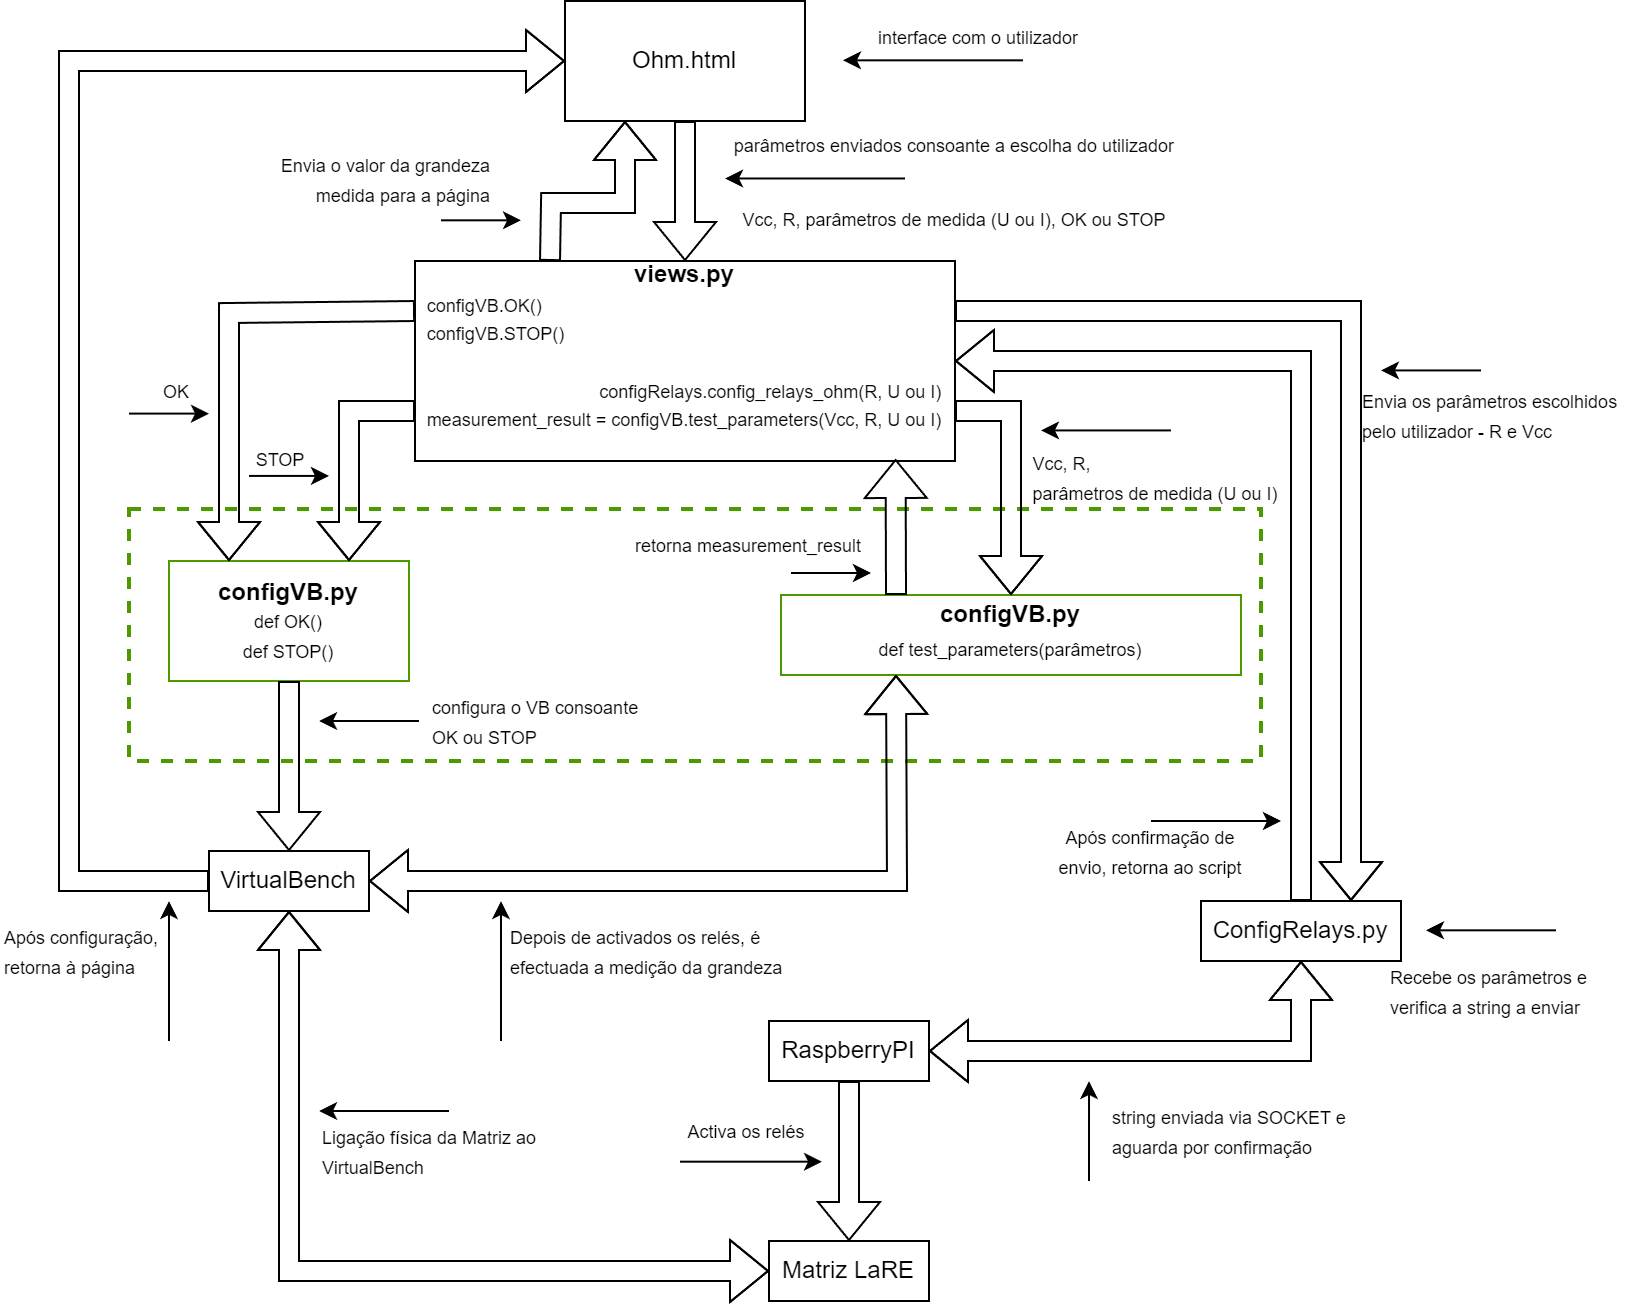
\includegraphics[width=1\textwidth]{figures/ohm_diagrama.drawio.png}
	\caption{Fluxograma/Esquema da experiência Lei de Ohm [REVER]}
	\label{fig:fluxohm}
\end{figure}

\subsubsection{Comunicação entre a página \textit{ohm.html} e o \textit{script views.py}}
De uma forma geral, a comunicação entre a página \textit{ohm.html} e o \textit{script views.py}, está representada esquematicamente na Figura \ref{fig:fluxohmpormenor}.

Entre estes dois ficheiros há envio/recepção de parâmetros.

O envio dos parâmetros da página \textit{ohm.html} é feito da forma como indica a Listagem \ref{lst:exemploenvioparametros}.
%, é feita da forma apresentada na Listagem \ref{lst:exemploenvioparametros}:

\begin{figure}[hbtp]
	\centering
	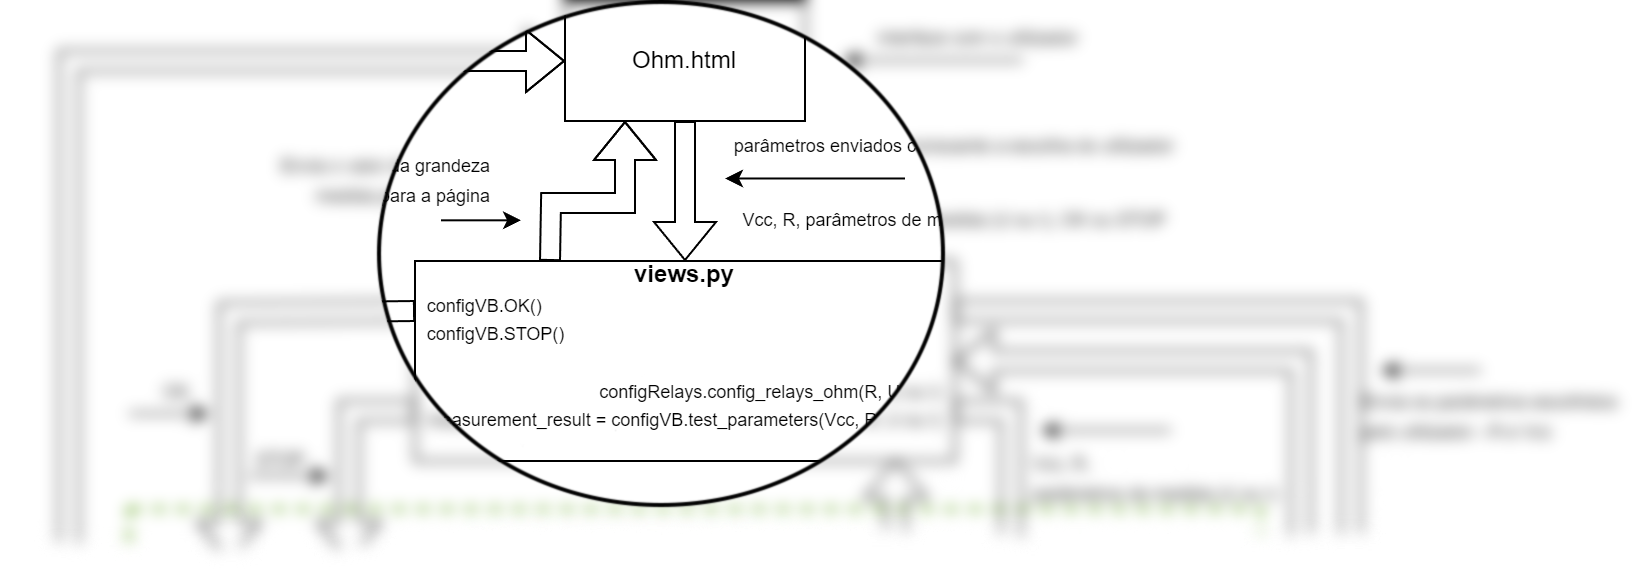
\includegraphics[width=1\textwidth]{figures/ohm_diagrama_pormenor.drawio.png}
	\caption{Fluxograma da comunicação entre a página ohm.html e o script views.py [REVER]}
	\label{fig:fluxohmpormenor}
\end{figure}

\begin{center}
	\begin{minipage}{0.7\linewidth}
		\begin{lstlisting}[language=Html, caption=Exemplo de envio de parâmetros da página \textit{ohm.html} para o \textit{script views.py}, label=lst:exemploenvioparametros]
		(...)
		const url = 
		`/config_VirtualBench?parameter1=${variavel_1}&parameter2=${variavel2}&parameter3=${variavel3}`
		(...)
	\end{lstlisting}
	\end{minipage}
\end{center}

Do lado do servidor (\textit{script views.py}) os parâmetros são recebidos da forma como se pode ver na Listagem \ref{lst:exemplorecepcaoparametros}:
\begin{center}
	\begin{minipage}{1\linewidth}
		\begin{lstlisting}[language=Python, caption=Exemplo da recepção dos parâmetros no \textit{script views.py} enviados da página \textit{ohm.html}, label=lst:exemplorecepcaoparametros]
			(...)
			@views.route('/config_VirtualBench', methods=['GET', 'POST'])
			@login_required
			def config_VirtualBench():
				try:
					Vcc = request.args.get('parametro2', 0, int)
					Resistance = request.args.get('parametro3', 0, int)
					measure_parameter = request.args.get('parametro1', 0, str)
			(...)
		\end{lstlisting}
	\end{minipage}
\end{center}

A página que é apresentada ao utilizador está representada na Figura \ref{fig:pagohm} e com mais pormenor na Figura \ref{fig:introohm}.
\begin{figure}[hbtp]
	\centering
	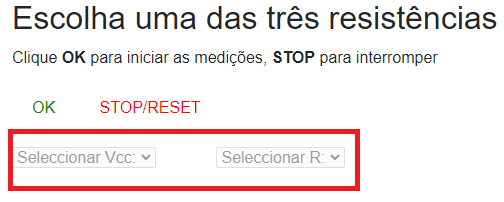
\includegraphics[width=0.7\textwidth]{figures/parametros_desabilitados.png}
	\caption{Página de entrada - \textit{ohm.html}}
	\label{fig:introohm}
\end{figure}

Como exemplo, os selectores dos parâmetros ``$V_{CC}$'' e ``R'' estão inicialmente desabilitados. Seleccionando ``OK'' as opções ficam disponíveis, como se pode ver na Figura \ref{fig:pagohm}. Neste caso, o respectivo parâmetro é enviado para o \textit{script} \textit{views.py}. No caso de os selectores estarem habilitados, ao carregar no botão ``STOP'', os selectores ficam desabilitados.

Do lado do \textit{script} \textit{views.py}, o parâmetro é recebido e, consoante o valor, são executadas as funções necessárias. Através da Listagem \ref{lst:recepcaoparametros} pode ver-se que, quando é recebido o parâmetro ``OK'', é chamada a função \textit{OK()} do \textit{script} \textit{configVB.py}. O procedimento é em tudo idêntico quando é seleccionado o parâmetro ``STOP''.

\begin{minipage}{0.9\linewidth}
	\begin{lstlisting}[language=python, caption=Recepção de parâmetros enviados de \textit{ohm.html}, label=lst:recepcaoparametros]
	(...)
	configOK = request.args.get('habilitar_parameter', None, bool)
	(...)
	if configOK == True:
        configVB.OK()      
    elif configSTOP == True:
        configVB.STOP()	
	(...)
	\end{lstlisting}
\end{minipage}

O envio dos restantes parâmetros, $V_{CC}$, R, medição de corrente (I) ou tensão (U) é feito de forma idêntica.

Quando se trata de enviar o resultado das medições para a página \textit{ohm.html}, a comunicação é feita da forma como se pode ver nas Listagens \ref{lst:envioresultados} e \ref{lst:recepcaoresultados}:
\begin{center}
	\begin{minipage}{0.7\linewidth}
		\begin{lstlisting}[language=python, caption=Envio de resultados do servidor (\textit{views.py}) para a página \textit{ohm.html}, label=lst:envioresultados]
			(...)
			return jsonify({'measurement_result': measurement_result})
			(...)
	\end{lstlisting}
	\end{minipage}
\end{center}

\begin{center}
	\begin{minipage}{0.7\linewidth}
		\begin{lstlisting}[language=html, caption=Recepção de resultados na página \textit{ohm.html}, label=lst:recepcaoresultados]
			(...)
			fetch(url)
			.then((response) => response.json())
		.then((data) => {
		  document.getElementById("current-measure").innerHTML =
			data.measurement_result + " mA";
			(...)
			\end{lstlisting}
	\end{minipage}
\end{center}

\subsubsection{O \textit{script configVB.py}}
\textbf{Este script poderá eventualmente ficar enquadrado numa secção a criar, denominada ``Descrição dos scripts'' ou então, na descrição da experiência lei de ohm.}
Neste \textit{script} fazem-se as configurações do \acrshort{virtualbench} e a construção do gráfico final e contém quatro funções referenciadas OU NÃO na Secção \textbf{SECÇÃO}:
\begin{itemize}
	\item \textit{OK()};
	\item \textit{STOP()};
	\item \textit{test\_parameters(Vcc:int, R:int, measure\_parameter:str)};
	\item \textit{plot\_graphic(current\_measurements, voltage\_measurements)}.
\end{itemize}

A função ``OK()'' é chamada quando o utilizador selecciona o botão ``OK'' na página \textit{ohm.html}. É responsável por activar a fonte de alimentação de \SI{12}{\volt} do \acrshort{virtualbench} e habilitar os selectores dos parâmetros $V_{CC}$ e R.

A função ``STOP()'' é chamada quando o utilizador selecciona o botão ``STOP'' na página \textit{ohm.html} e funciona como uma espécie de \textit{RESET}. Esta função é responsável por desactivar e libertar todas saídas do \acrshort{virtualbench}, assim como os instrumentos e o próprio \acrshort{virtualbench}. Os selectores dos parâmetros $V_{CC}$ e R também são desabilitados.

%é chamado no \textit{script views.py}, consoante o valor do parâmetro recebido. A Figura \ref{fig:cutconfigVB} representa o diagrama de blocos do \textit{script}.

Para se perceber melhor a função deste \textit{script} e das funções descritas em cima, importa clarificar o modo de funcionamento e a implementação da página \textit{ohm.html}.

Como se pode ver nas Figuras \ref{fig:pagohm} e \ref{fig:pagohmabc}, representadas na Secção \ref{sec:lei_ohm}, a página \textit{ohm.html} é composta por um formulário que permite ao utilizador escolher os parâmetros $V_{CC}$ e R, assim como a medição a efectuar - corrente ou tensão e a construção do gráfico.

De forma a prevenir qualquer descuido ou erro de utilização, os parâmetros escolhidos só serão efectivamente enviados para o servidor \textit{Flask} - (\textit{views.py}) e a medição efectuada quando:
\begin{enumerate}
	\item Seleccionar o botão ``OK'' que habilita os selectores;
	\item Escolher ambos os parâmetros - $V_{CC}$ e R;
	\item Clicar no link ``Medir tensão'' ou ``Medir corrente''.
\end{enumerate}

A verificação dos erros e escolha de parâmetros é feita na página \textit{ohm.html}, tal como se pode ver pela Listagem \ref{lst:erro} e pelo exemplo da Figura \ref{fig:??} .

\begin{center}
	\begin{minipage}{0.7\linewidth}
		\begin{lstlisting}[language=html, caption=Erro na página \textit{ohm.html}, label=lst:erro]
		(...)
        if (Vcc === "0" || Resistance === "0") {
          alert("Tem de primeiro seleccionar os valores de Vcc e R!");
          return;
        }
		(...)
	\end{lstlisting}
	\end{minipage}
\end{center}

\hrule

\subsubsection{Fontes de alimentação - a incluir no hardware}
O \acrshort{lare} utiliza várias tensões de alimentação:
\begin{itemize}
	\item \SI{12}{\volt} - para alimentar os relés e os \textit{drivers} dos relés - ULN2003;
	\item \SI{5}{\volt} - para alimentar os registos de deslocamento - 74HC595;
	\item fonte tensão variável (\acrshort{cc}) para alimentar a experiência da Lei de \textit{Ohm};
	\item fonte tensão \acrshort{ca} para alimentar as experiências de filtros rectificação.
\end{itemize}

No que concerne à fonte de alimentação \acrshort{ca}, esta foi implementada de forma independente, ou seja, não depende do \acrshort{virtualbench}. \textbf{Falar sobre a fonte de alimentação variável e a fonte de alimentação \acrshort{ca}. Colocar a foto do esquema e explicar como se faz a rectificação, cálculos inclusive. Talvez referir o facto de que depende da qualidade e valores dos transformadores e depois concluir com os valores deste caso, pode-se refferir que relativamente à fonte AC, só está disponível a fonte do gerador de sinal do VB e é mais fácil controlar através da fonte externa projectada.}

Tal como pode ser visto na Figura \ref{fig:fontes_VB}, o \acrshort{virtualbench} possui três fontes de alimentação continua: \SI{6}{\volt}, \SI{25}{\volt} e \SI{-25}{\volt}\footnote{No contexto do \acrshort{lare}, a fonte de tensão de \SI{-25}{\volt} não foi usada}. 

\begin{figure}[hbtp]
	\centering
	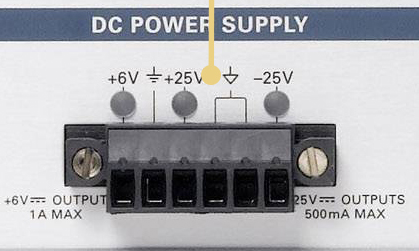
\includegraphics[width=1\textwidth]{figures/fontes_VB.png}
	\caption{Fontes de tensão contínua \acrshort{virtualbench}}
	\label{fig:fontes_VB}
\end{figure}

Para a implementação da experiência da Lei de \textit{Ohm} e como já foi referido em cima, os circuitos integrados necessitam de \SI{5}{\volt} e \SI{12}{\volt} de alimentação e \SI{6}{\volt} variáveis para as medições das tensões e correntes nas resistências. Como só duas fontes de alimentação são controláveis, optou-se por configurar a fonte de \SI{25}{\volt} conforme representado no esquema da Figura \ref{fig:fontes_VB}.

Como se pode ver na Figura , os selectores estão desabilitados e os relés nao estão alimentados porque isso é feito através da fonte do VB e do LM317

Já se viu (\textbf{refirerir a secção}) que na experiência da Lei de \textit{Ohm}, o utilizador selecciona os valores da tensão e resistência através de um formulário, representado na página \textit{ohm.html} da forma como se pode ver na Listagem \ref{lst:formularioescolha}.

\begin{center}
	\begin{minipage}{0.7\linewidth}
		\begin{lstlisting}[language=html, caption=Formulário de escolha na página \textit{ohm.html},label=lst:formularioescolha]
			(...)
			<div style="display: inline-block; width: 200px">
      <select id="selectVcc" disabled>
        <option value="0">Seleccionar V<sub>cc</sub>:</option>
        <option value="1">1</option>
        <option value="2">2</option>
        <option value="3">3</option>
        <option value="4">4</option>
        <option value="5">5</option>
      </select>
    </div>

    <div style="display: inline-block; width: 200px">
      <select id="selectR" disabled>
        <option value="0">Seleccionar R:</option>
        <option value="1">1</option>
        <option value="2">1.1</option>
        <option value="3">1.5</option>
      </select>
			(...)
	\end{lstlisting}
	\end{minipage}
\end{center}

No entanto, optou-se por adicionar à página \textit{ohm.html} um botão ``OK'' que, ao ser seleccionado, activa os selectores e envia os parâmetros para o servidor. O \textit{script} \textit{configVB.py} é chamado no \textit{script views.py}, consoante o valor do parâmetro recebido. A Figura \ref{fig:cutconfigVB} representa o diagrama de blocos do \textit{script}.

explicar porque se optou por colocar o botão ``OK'' e não enviar os parâmetros automaticamente, e só efectuar a medição quando se clicar no link medir.

Aqui vai ter de seexplicar porque se activa o OK. O Ok activa, antes de mais, a fonte de 12V que vai alimentar os integrados e, através do LM317, a fonte de 5V. 

Só depois os formulários são activos, permite seleccionar os valores e só depois é que o uti.lizador pode clicar no link medir.
Isto permite que o utilizador tenha mais controlo sobre a experiência.

Explicar porque é chamado o \textit{script configVB.py} e o que faz cada funlção
OK faz....
STOP faz....

Explicar porque os selectores estão desabilitados, foi o critério utilizado para realizar a configuração inicial do VB. Assim, quando dse carrega no "OK", habilitam-se os selectores e ao mesmo tempo, enviam-se os parâmetros para o servidor, de forma a configurar o VB. Que tipo de configuração se faz? Activa-se a fonte de 12V - colocar exemplo do programa e referenciar esquema de ligações - e alimentam-se os integrados de 12V e 5V - colocar ou referenciar o esquema

Na Secção anterior descreveu-se o processo de comunicação entre a página \textit{ohm.html} e o \textit{script views.py} (servidor).

%Se os parâmetros forem correctamente recebidos no \textit{script views.py} (servidor) são chamados dois \textit{scripts}, que executaram a função : \textit{configVB.py} e \textit{configRelays.py}. 

O primeiro a ser chamado, como pode ser vist
\begin{figure}[hbtp]
	\centering
	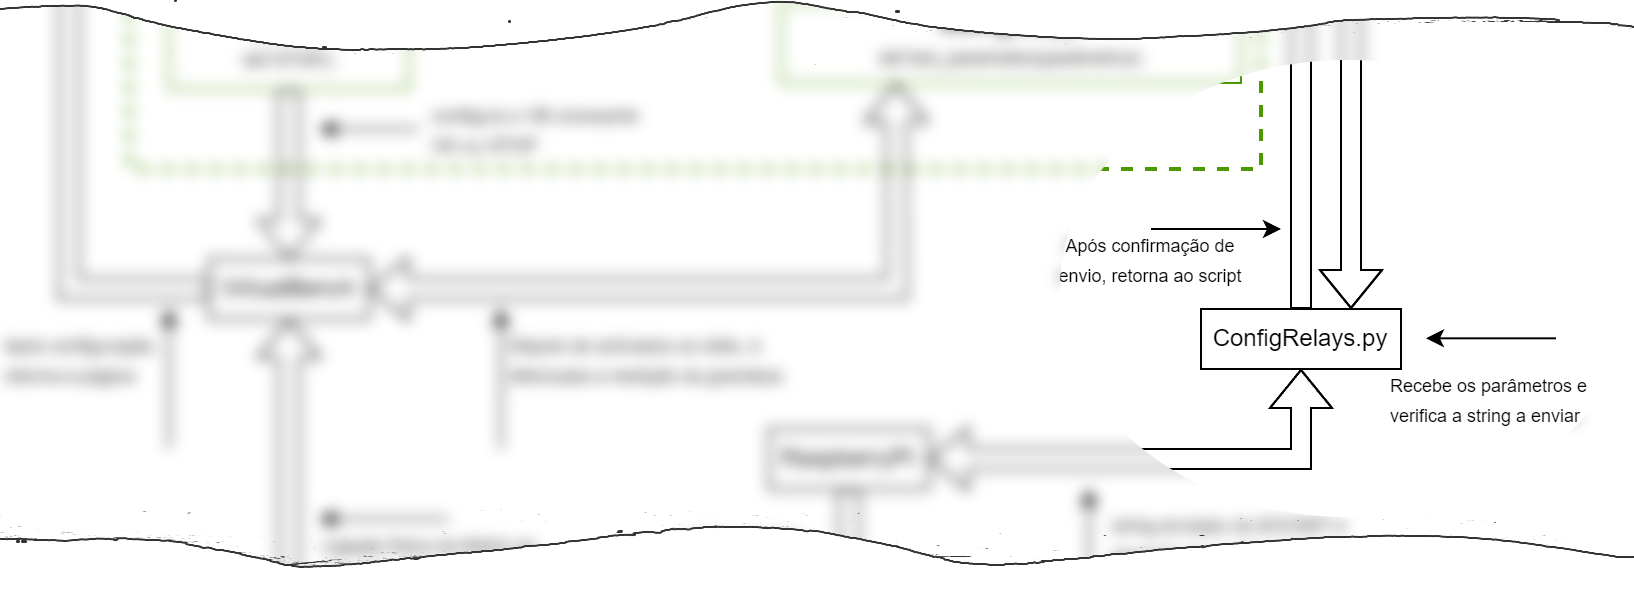
\includegraphics[width=1\textwidth]{figures/ohm_diagramaCUTRelay.drawio.png}
	\caption{\textit{Script configRelays.py}}
	\label{fig:cutconfigRelays}
\end{figure}

\section{qualquer coisa que ainda não sei o quê}

Após análise e estudo da informação presente no \textit{site} do \textit{Flask} e nos tutoriais mencionados em cima, definiu-se e implementou-se a página de autenticação no ficheiro \textit{auth.py}, tal como pode ser visto na Figura \ref{fig:paglogin}:

\begin{figure}[hbtp]
	\centering
	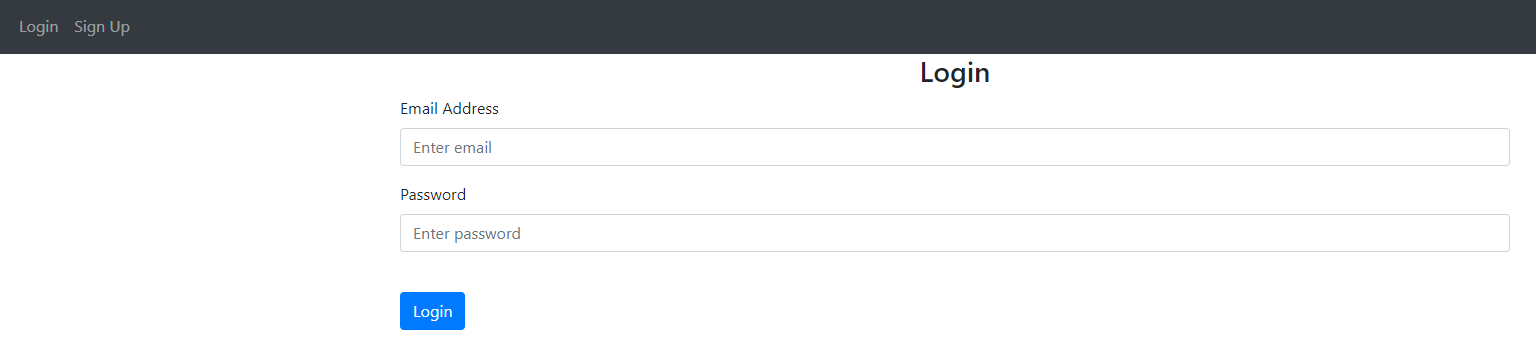
\includegraphics[width=1\textwidth]{figures/login.png}
	\caption{Página de \textit{login}}
	\label{fig:paglogin}
\end{figure}

\begin{figure}[hbtp]
	\centering
	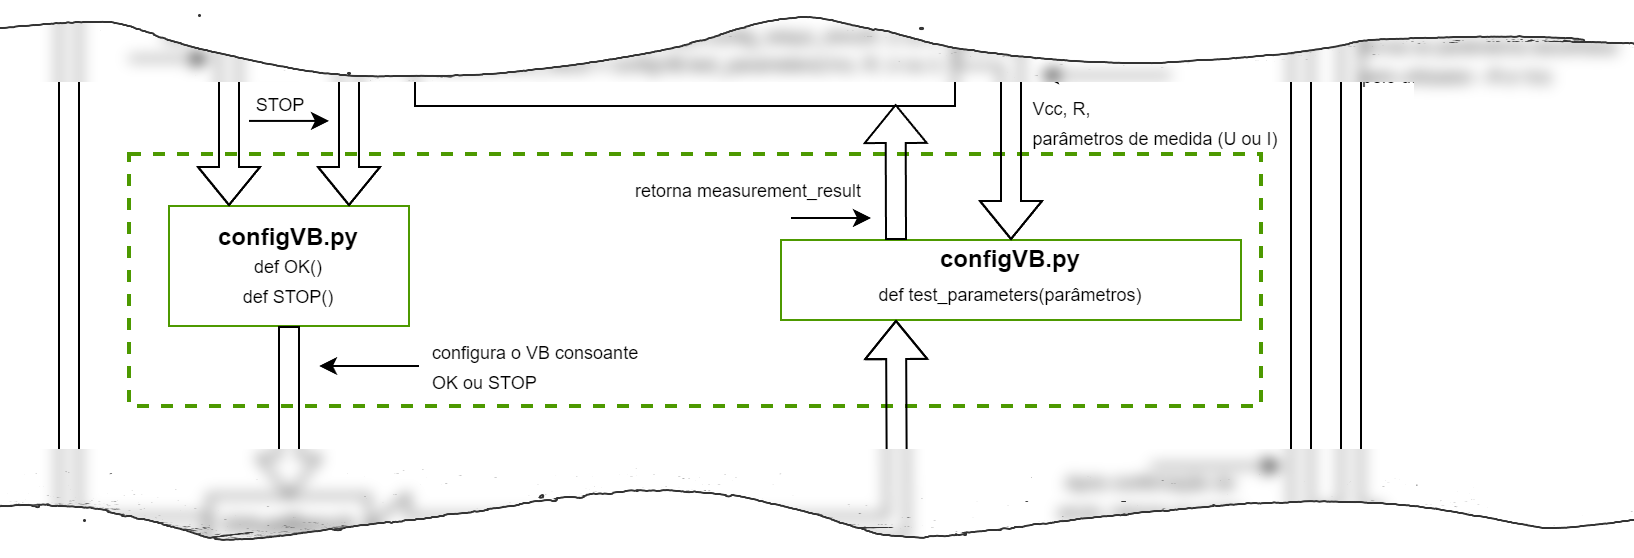
\includegraphics[width=1\textwidth]{figures/ohm_diagramaCUT.drawio.png}
	\caption{caralho}
	\label{fig:diagramaCUT}
\end{figure}

Um exemplo de como foi implementada a função \textit{login}() está representada na Listagem \ref{lst:exemplologin} e a rota está definida para a página \textit{/login}, como apresentado na mesma Figura, linha 17.

Os dados de \textit{login} e registo são guardados na directoria \textit{instance}, ficheiro \textit{database.db}.

Além da rota definida para o \textit{login}, as outras rotas definidas no ficheiro \textit{auth.py} foram as \textit{sign-up} e \textit{logout}. A estrutura base da função \textit{login}, representada na Listagem \ref{lst:exemplologin}, é idêntica para as restantes, sendo que ``/\textit{login''} representa a rota especificada, dentro da função há o código especifico inerentes a cada função e o \textit{return render\_template} indica qual a página a ser renderizada.

A juntar às páginas que compõem a estrutura base do \textit{site}, representadas na Figura \ref{fig:estruturapastas}, há ainda a juntar as páginas que permitem ao utilizador interagir com as experiências do \acrshort{lare}. Neste caso, serão cinco páginas, correspondentes aos 5 circuitos definidos na Secção \ref{sec:solucaoproposta}.

O menu de escolha foi retirado do \textit{site} \href{https://www.w3schools.com/howto/howto_js_vertical_tabs.asp}{\textit{w3schools}} e modificado de acordo com as necessidades do projecto, tal como pode ser visto na Figura \ref{fig:pagmenu}.

\begin{figure}[hbtp]
	\centering
	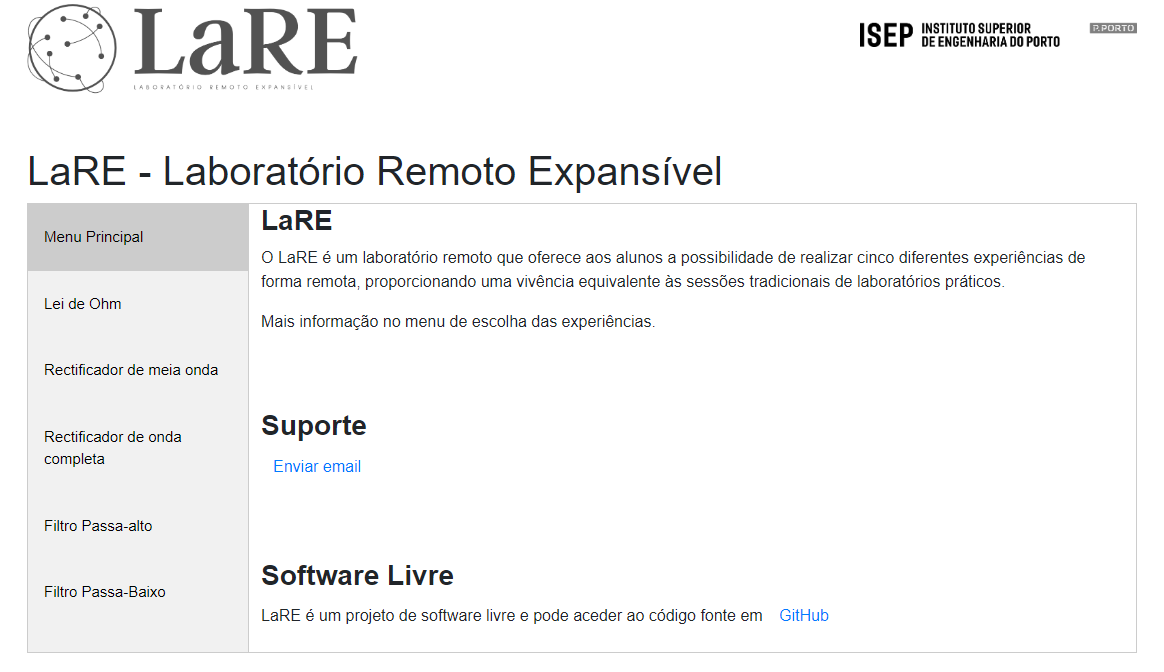
\includegraphics[width=1\textwidth]{figures/menupage.png}
	\caption{Página de menus}
	\label{fig:pagmenu}
\end{figure}

As páginas referentes às experiências seguem a mesma estrutura de menus.

\sout{Uma das partes mais cruciais e que levantou mais dificuldades foi a comunicação e o envio de parâmetros entre as páginas \acrshort{html} e o \textit{Flask}.}

Esta matriz, que inclui os circuitos definidos na Secção \ref{sec:solucaoproposta}, assim como a alimentação e as ligações ao \gls{RaspberryPI}, compõe as 5 experiências.

Esta matriz é composta por 3 placas:
\begin{itemize}
	\item Alimentação:
	      \begin{itemize}
		      \item Transformador;
		      \item Fonte de tensão de \SI{5}{\volt};
	      \end{itemize}
	\item Circuito da Lei de Ohm;
	\item Circuitos de Rectificação e filtros:
	      \begin{itemize}
		      \item Rectificação de meia onda;
		      \item Rectificação de onda completa;
		      \item Filtro passa-baixo;
		      \item filtro passa-alto.
	      \end{itemize}
\end{itemize}